% Use only LaTeX2e, calling the article.cls class and 12-point type.

\documentclass[11pt]{article}
\usepackage[round,semicolon]{natbib}
\usepackage[margin=1.4in]{geometry}
\usepackage{kpfonts}

\usepackage{seqsplit}
\usepackage{placeins}

\usepackage{newfloat}
\usepackage[labelfont=bf]{caption}
\usepackage{nameref}
\usepackage{rotating}
\usepackage{color}
\usepackage{float}

\setcounter{topnumber}{8}
\setcounter{bottomnumber}{8}
\setcounter{totalnumber}{8}

\usepackage{newfloat}
\DeclareFloatingEnvironment[name={Figure}]{suppfigure}
\renewcommand{\thesuppfigure}{S\arabic{suppfigure}}

\definecolor{darkblue}{rgb}{0, 0.0, 0.6}

\usepackage{hyperref}
\hypersetup{colorlinks,citecolor=blue,linkcolor=blue,urlcolor=blue}

\usepackage{seqsplit}

\usepackage{array}
\newcolumntype{R}[1]{>{\raggedright\arraybackslash}p{#1}}
\newcolumntype{C}[1]{>{\centering\let\newline\\\arraybackslash\hspace{0pt}}m{#1}}

\newcommand{\comment}[1]{{\color{red}[\textsl{#1}]}}

\usepackage{setspace}

\renewcommand{\topfraction}{1}
\renewcommand{\bottomfraction}{1}
\renewcommand{\textfraction}{0}
\renewcommand{\floatpagefraction}{1}

%\renewcommand{\abstractname}{\large SUMMARY}


\title{Quantifying the ease of viral escape from broad and narrow antibodies to an H1 influenza hemagglutinin} 

\author
{Michael B. Doud$^{1,2,3,\dagger}$, Juhye M. Lee$^{1,2,3,\dagger}$, and Jesse D. Bloom$^{1,2,*}$\\
\\
\scriptsize{$^1$Basic Sciences and Computational Biology Program, Fred Hutchinson Cancer Research Center}\\
\scriptsize{$^2$Department of Genome Sciences and $^3$Medical Scientist Training Program, University of Washington} \\
\scriptsize{Seattle, WA, USA} \\
\scriptsize{$^{\dagger}$These authors contributed equally} \\
\scriptsize{$^*$Correspondence: \href{jbloom@fredhutch.org}{jbloom@fredhutch.org}}
}

\date{}


\begin{document}

\maketitle
\onehalfspacing

\begin{abstract}
Influenza virus can completely escape most antibodies with single mutations.
However, rare antibodies broadly neutralize many viral strains.
It is unclear how easily influenza virus might escape such antibodies if they became widespread due to therapeutic use or vaccination.
Here we map all single amino-acid mutations that increase resistance to broad antibodies targeting an H1 hemagglutinin.
Crucially, our approach not only identifies antigenic mutations but also quantifies their effect sizes.
All antibodies select mutations, but the effect sizes vary widely. 
The virus can escape a broad antibody targeting hemagglutinin's receptor-binding pocket the same way it escapes narrow strain-specific antibodies: via single mutations with huge effects.   
In contrast, broad antibodies targeting hemagglutinin's stalk only select mutations with small effects. 
Therefore, antibody breadth is not necessarily an indicator of the difficulty of viral escape.
Broad antibodies targeting hemagglutinin's stalk are quantifiably harder to escape than antibodies targeting hemagglutinin's head or receptor-binding pocket.
\end{abstract}

\section*{INTRODUCTION}
Nearly all viruses show some antigenic variation.
However, the extent of this variation ranges widely.
For instance, although both measles virus~\citep{birrer1981antigenic,ter1981antigenic} and polio virus~\citep{crainic1983natural,diamond1985antigenic,drexler2014robustness} exhibit antigenic variation, the magnitude of this variation is small. 
Therefore, immunity to these viruses is lifelong~\citep{panum1847iagttagelser,salk1984one}.
In contrast, human influenza virus exhibits much more antigenic variation.
So although infection with an influenza virus strain provides long-term immunity to that exact strain~\citep{davies1982christ,yu2008neutralizing}, the virus's rapid antigenic evolution erodes the effectiveness of this immunity to that strain's descendants within four to seven years~\citep{couch1983immunity}.

One possible reason that viruses exhibit different amounts of antigenic variation is that they have disparate evolutionary capacities to escape the immunodominant antibodies generated by natural immune responses~\citep{lipsitch2007patterns,cobey2014pathogen,fulton2015mutational}.
According to this explanation, human influenza virus undergoes rapid antigenic drift because most neutralizing antibodies target epitopes on the viral hemagglutinin (HA) protein that are highly tolerant of mutational change.
This explanation is supported by classic experiments showing that it is easy to select viral mutants that escape most antibodies~\citep{yewdell1979antigenic,webster1980determination}, as well as by the observation that mutations that alter antigenicity arise frequently during influenza's evolution globally~\citep{koel2013substitutions,chambers2015identification,petrie2016antibodies,neher2016prediction} and within individual humans with long-term infections~\citep{xue2017parallel}.
A corollary of this explanation is that influenza virus's capacity for antigenic drift would be reduced if most antibodies instead targeted epitopes that were less mutationally tolerant.

Verifying this corollary has become of practical importance with the discovery of broadly neutralizing antibodies against influenza virus.
These antibodies typically target conserved epitopes in HA's stalk~\citep{sui2009structural,ekiert2009antibody,corti2011neutralizing} or receptor-binding pocket~\citep{lee2012heterosubtypic,ekiert2012cross}, and neutralize a wide range of viral strains.
Broad antibodies are usually less abundant in human serum than antibodies to antigenically variable epitopes on the head of HA~\citep{ellebedy2014induction,andrews2015immune}.
However, major efforts are underway to elicit broad antibodies by vaccination or administer them directly as therapeutics~\citep{krammer2015advances,corti2017tackling}.

If these efforts succeed, the epitopes of broad antibodies will be under strong antigenic selection in human influenza virus.
Might such selection then drive antigenic variation in these epitopes?
There is precedent for the idea that the immune status of the host population can shape influenza virus evolution: the virus undergoes faster antigenic drift in long-lived humans that accumulate immune memory than in short-lived swine that are mostly naive~\citep{sheerar1989antigenic,luoh1992hemagglutinin}, and poultry vaccination may accelerate antigenic drift of avian influenza~\citep{lee2004effect,cattoli2011antigenic}.
But alternatively, perhaps broad antibodies are broad because the virus has difficulty escaping them regardless of selection from host immunity.

So far, there is limited data to distinguish between these possibilities.
Several studies have shown that the head domain of HA is less mutationally tolerant than the stalk domain where many broad antibodies bind~\citep{thyagarajan2014inherent,wu2014high,heaton2013genome}.
However, these studies did not select for actual antibody escape, so it is difficult to relate their measurements to the virus's evolutionary capacity under immune selection.
Other work has shown that it is possible to select antigenic mutants with broad antibodies~\citep{yoshida2009cross,chai2016two}, demonstrating that these epitopes are not entirely refractory to change.
But given that antibodies can select some antigenic variation even in measles virus~\citep{birrer1981antigenic,ter1981antigenic} and polio virus~\citep{crainic1983natural,diamond1985antigenic}, the existence of selectable mutations does not necessarily imply that influenza virus can escape broad antibodies with the same ease that it drifts away from narrow strain-specific ones.
The fundamental problem is that existing studies have not quantified the ease of viral escape in a way that can be compared across antibodies in an apples-to-apples fashion.

Here we systematically quantify the results of selecting all single amino-acid mutations to an H1 HA with several broad and narrow antibodies.
Critically, our approach quantifies the \emph{magnitude} of the antigenic effect of every mutation in a way that can be directly compared across antibodies.
We find that even the broadest antibodies select antigenic mutations.
However, the magnitudes of the antigenic effects vary greatly across antibodies.
Single mutations make the virus completely resistant to both narrow strain-specific antibodies and a broad antibody against the receptor-binding pocket.
But no single mutation does more than modestly increase the virus's resistance to broad antibodies against the HA stalk.
Therefore, broad anti-stalk antibodies are quantifiably more resistant to viral escape via single amino-acid mutations than the other antibodies tested here. 


\section*{RESULTS}
\label{sec:results}

\subsection*{An approach to quantify the fraction of virions with each mutation that escape antibody neutralization}
We can visualize the outcome of antibody selection on viral populations containing antigenic mutations as in Figure~\ref{fig:fracsurvive_example}.
If a mutation strongly escapes neutralization, then all virions with this mutation will survive antibody treatment at a concentration where other virions are mostly neutralized (Figure~\ref{fig:fracsurvive_example}A).
This escape is manifested by a large rightward shift in the neutralization curve for the mutant (Figure~\ref{fig:fracsurvive_example}B).
If we draw vertical lines through the overlaid neutralization curves, we can calculate the fraction of virions with each mutation that escape neutralization at each antibody concentration (Figure~\ref{fig:fracsurvive_example}B).
These fractions can be represented using logo plots, where the height of each letter is proportional to the fraction of virions with that amino acid at a site that survive the antibody (Figure~\ref{fig:fracsurvive_example}C).
In these logo plots, large letters correspond to strong escape mutations. 

\begin{figure}
\centerline{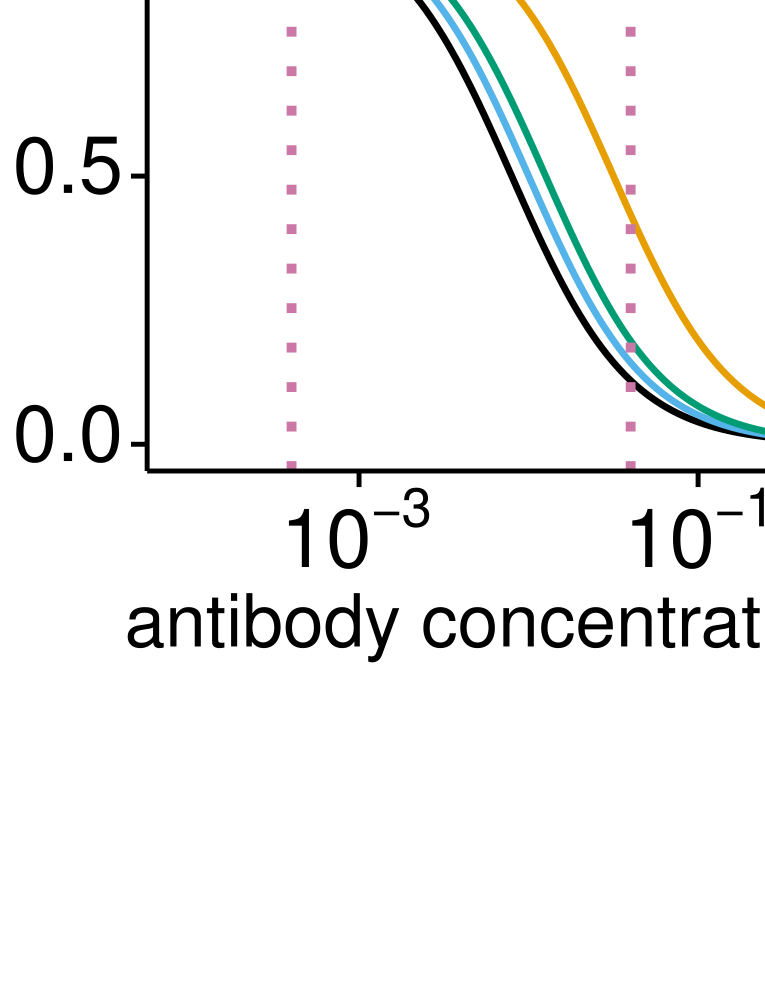
\includegraphics[width=\textwidth]{figs/fracsurvive_example/fracsurvive_fig.pdf}}
\caption{\label{fig:fracsurvive_example}
{\bf Quantifying the fraction of virions with each mutation that escape antibody neutralization.}
This figure shows hypothetical data for four viral variants: wildtype and three mutants.
(A) Virions with the V1K mutation (orange) completely survive an antibody concentration where most other virions are neutralized.
(B) This resistance is manifested by a large shift in V1K's neutralization curve.
(C) For each dotted vertical line drawn through the neutralization curves in (B), we calculate the fraction of virions with that mutation that survive the antibody, and indicate this fraction by the height of the letter corresponding to that amino acid at that site.
(D-F) Similar data to the first three panels, but now V1K has only a small antigenic effect, and so only modestly increases the fraction of virions that survive antibody treatment.
}
\end{figure}

Now consider the case where a mutation has just a small antigenic effect, and so only slightly increases the fraction of virions that escape neutralization (Figure~\ref{fig:fracsurvive_example}D).
In this scenario, the neutralization curve shifts only slightly to the right (Figure~\ref{fig:fracsurvive_example}E).
In the logo plot representation, the antigenic mutation is only slightly larger than other amino acids (Figure~\ref{fig:fracsurvive_example}F), since possessing the mutation only modestly increases the chance that a virion survives antibody treatment.
These logo plots therefore provide a way to both identify escape mutations and quantify the magnitudes of their antigenic effects in a way that is directly comparable across antibodies.

Our goal is to determine the fraction of mutant virions that escape antibody neutralization for \emph{all} mutations to influenza HA.
In other words, we want to generate logo plots like those in Figure~\ref{fig:fracsurvive_example} for every amino acid at every site in HA.
One way to do this would be to measure individual neutralization curves for each of the $19\times565 = 10,735$ single amino-acid mutants of the 565-residue HA protein.
However, individually creating and assaying that many viral mutants would be time-consuming and expensive.
Fortunately, we have recently shown that antibody selection on all viral mutations can be assayed in a single experiment using an approach termed mutational antigenic profiling~\citep{doud2017complete,dingens2017comprehensive}.
This approach involves generating viral libraries containing all mutations to the protein of interest (in this case, HA), selecting these viruses with or without antibody, and then using an accurate deep-sequencing method to determine the relative frequencies of each mutation.

These frequencies can be analyzed to calculate the fraction of virions with each mutation that survive antibody treatment.
Specifically, the deep sequencing determines the frequencies of virions carrying amino-acid $a$ at site $r$ in the antibody-selected and mock-selected conditions, which we denote as $\rho_{r,a}^{\rm{selected}}$ and $\rho_{r,a}^{\rm{mock}}$, respectively.
We can also measure the total fraction of the viral library that survives the antibody treatment, which we denote as $\gamma$.
The fraction of variants with amino-acid $a$ at site $r$ that survive antibody selection is then simply 
\begin{equation}
\label{eq:fracsurvive}
F_{r,a} = \gamma \times \frac{\rho_{r,a}^{\rm{selected}}}{\rho_{r,a}^{\rm{mock}}}.
\end{equation}
For instance, in Figure~\ref{fig:fracsurvive_example}A, the frequency of virions with the orange mutation is $\rho_{r,a}^{\rm{selected}} = \frac{4}{7}$ in the antibody-selected condition and $\rho_{r,a}^{\rm{mock}} = \frac{4}{16}$ in the mock-selected condition.
The overall fraction of virions that survive the antibody in Figure~\ref{fig:fracsurvive_example}A is $\gamma = \frac{7}{16}$.
Therefore, we use Equation~\ref{eq:fracsurvive} to calculate that the fraction of variants with the orange mutation that survive the selection is $F_{r,a} = \frac{7}{16} \times \frac{4/7}{4/16} = 1$.
Performing the analogous calculation for Figure~\ref{fig:fracsurvive_example}D correctly determines that fraction of virions with the orange mutation that survive the antibody is only 0.5 for the scenario in that figure panel.
In most of the analyses of real data below, we will plot the fraction surviving \emph{above} the overall library average, which is
\begin{equation}
\label{eq:fracsurvive_above}
F_{r,a}^{\rm{aboveavg}} = \max\left(0, F_{r,a} - \gamma\right).
\end{equation}
We plot the fraction surviving above the library average rather than the raw fraction surviving since the former quantity more clearly accentuates antigenic mutations against the background of other mutations.
Details of how the calculations are extended to account for sequencing errors and sampling statistics are in the \nameref{sec:methods}.
Open-source software that performs all steps in the analysis beginning with the deep sequencing data is available at \url{https://jbloomlab.github.io/dms_tools2/}.

\subsection*{Broad and narrow antibodies that neutralize influenza virus}
\comment{Juhye writes a draft of this section.}

% blurbs about the specific antibodies we use here:
C179 isolation and escape mutant selection \cite{okuno1993common}.
C179 structure with 1957 H2, binding data to many strains, and citations to older studies demonstrating C179 cross-neutralization to H1, H2, H5, H6, and H9:  \cite{dreyfus2013structure}.
FI6v3 was isolated... \cite{corti2011neutralizing}.
S139/1 isolation and selection of escape mutants from Aichi H3, Adachi H2, and WSN H1: \cite{yoshida2009cross}.
S139/1 structure with Victoria75 H3 and binding/neutralization data: \cite{lee2012heterosubtypic}.

\begin{figure}
\centerline{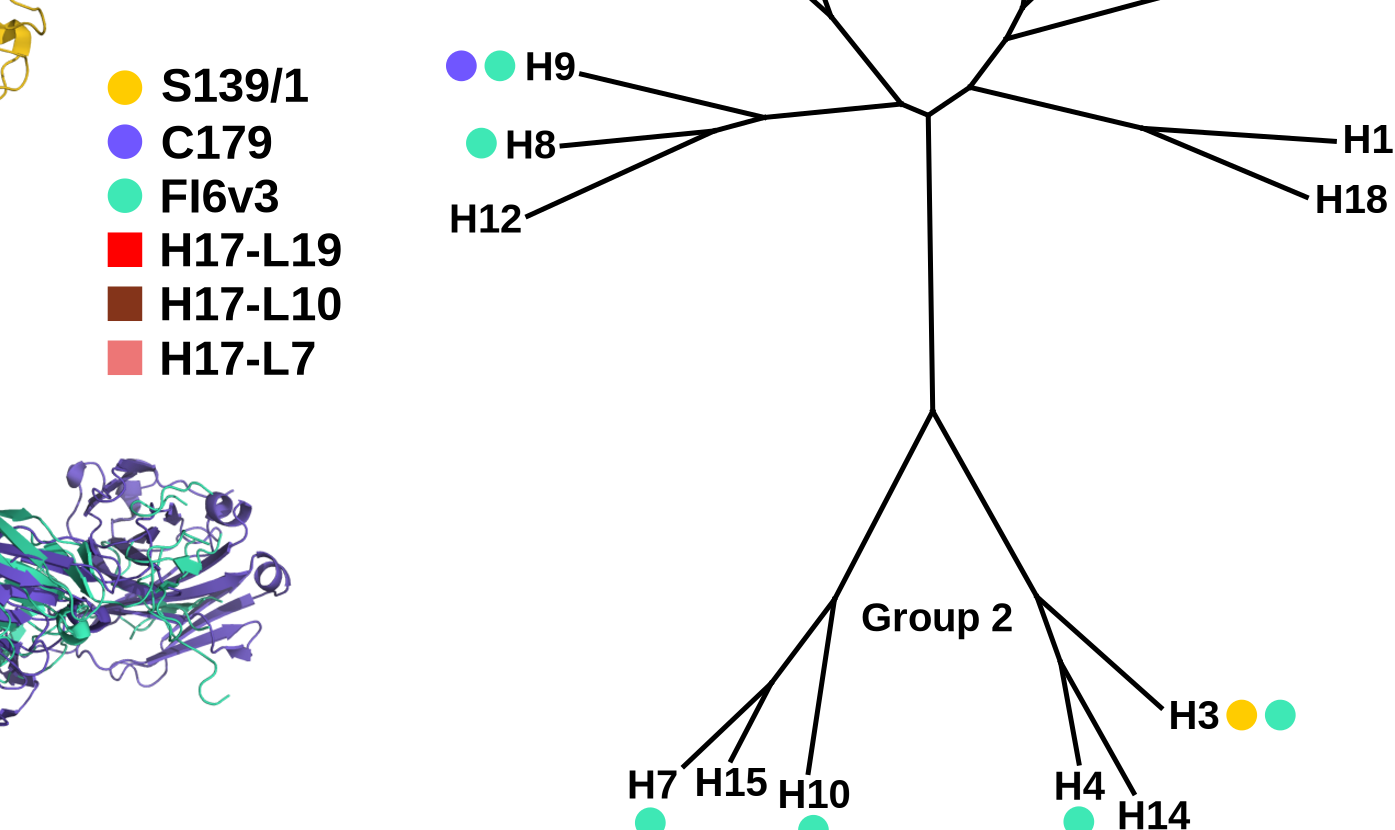
\includegraphics[width=\textwidth]{figs/antibody_summary_fig/Ab_summary.pdf}}
\caption{\label{fig:antibody_summary}
CAPTION
}
\end{figure}


\begin{figure}
\centerline{\includegraphics[width=0.8\textwidth]{figs/neutralization_curves/WT_neutralization_curves.pdf}}
\caption{\label{fig:neutcurves}
CAPTION
\comment{
Get rid of the panel numbers altogether and just have the antibody names.
}
}
\end{figure}

\subsection*{Quantifying the antigenic effects of all mutations selected by each antibody}
We performed mutational antigenic profiling using the three broadly neutralizing antibodies (FI6v3, C179, and S139/1) at the concentrations indicated in Figure~\ref{fig:neutcurves}, and analyzed the data to calculate the fraction of virions carrying each mutation that survived neutralization. 
All experiments were performed in full biological triplicate using three independently generated virus libraries carrying all amino-acid mutants to the HA of the A/WSN/1933 (H1N1) strain~\citep{doud2016accurate}, and in some cases we also included technical replicates with the same virus library.
We have previously described~\citep{doud2017complete} complete mapping of escape from the three strain-specific antibodies (H17-L19, H17-L10, and H17-L7) at the concentrations indicated in Figure~\ref{fig:neutcurves}, and we also re-analyzed those deep sequencing data to calculate the fraction of virions with each mutation that survived each selection.
The correlations among replicates are shown in Figure~\ref{suppfig:corr}.
For the remainder of this paper, we will refer to the median antigenic effect of each mutation taken across all replicates with that antibody at that concentration.


\comment{Jesse can work on a rough draft of this section.}

\begin{figure}
\centerline{\includegraphics[width=\textwidth]{figs/avgfracsurvive.pdf}}
\caption{
\label{fig:avgfracsurvive}
CAPTION
Figure~\ref{suppfig:maxfracsurvive} shows the fraction surviving for the single most strongly selected amino-acid mutation at each site.
}
\end{figure}

\subsection*{For all antibodies, the selected sites of escape occur in the antibody binding footprints}

\section*{DISCUSSION}
Some discussion

\clearpage

\section*{METHODS}
\label{sec:methods}
\subsection*{Antibodies}
FI6v3 was expressed and purified by the Fred Hutchinson Cancer Research Center protein expression core \comment{i think?}.
C179 was purchased from Takara Bio Inc (Catalog \# M145).
S139/1 heavy and light chain variable sequences were obtained from PDB ID 4GMS~\cite{lee2012heterosubtypic} and expressed and purified by the Fred Hutchinson Cancer Research Center protein expression core.

\subsection*{Mutant virus selections with antibody}
Library selections, deep sequencing, and computation of mutation differential selection were performed as previously described~\cite{doud2017complete}. Briefly, ...

\subsection*{Calculating the fraction of virions with each mutation that escapes antibody neutralization}
In prior mutational antigenic profiling work~\citep{doud2017complete,dingens2017comprehensive}, we calculated the differential selection on each mutation as the logarithm of its enrichment relative to wildtype in an antibody-selected sample versus a mock-selected control.
These \emph{mutation differential selection} values are useful for the analysis of individual experiments.
However, there is no natural way to compare these values across experiments with different antibodies at different concentrations, since the strength of differential selection depends on details of how the pressure is imposed.
We therefore developed the new approach in this paper to quantify the antigenic effect of a mutation in units that can be compared across antibodies and concentrations.

The general principle of the calculations is illustrated in Figure~\ref{fig:fracsurvive_example} and discussed in the first section of the \nameref{sec:results}.
Code that performs these calculations is included in the \texttt{dms\_tools2} software package~\citep{bloom2015software} which is available at \url{http://jbloomlab.github.io/dms_tools2}.


\subsection*{Data availability and source code}
Deep sequencing data are available from the Sequence Read Archive under BioSample accession (\comment{add this}).


\clearpage

\small
\subsection*{ACKNOWLEDGMENTS}
This work was supported by grants R01GM102198 and R01AI127893 from the NIGMS and NIAID of the NIH.
MBD was supported in part by training grant T32AI083203 from the NIAID of the NIH.
JML was supported in part by \comment{CIDID grant}.
The research of JDB is supported in part by a Faculty Scholar Grant from the Howard Hughes Medical Institute and the Simons Foundation.

\bibliographystyle{mbe}
\bibliography{references.bib}

\clearpage
\normalsize

\section*{Supplementary Material}
\FloatBarrier

\begin{suppfigure}
\centerline{\includegraphics[width=0.6\textwidth]{figs/corrs/site_correlations_bnAbs.pdf}}
\vspace{0.2in}

\centerline{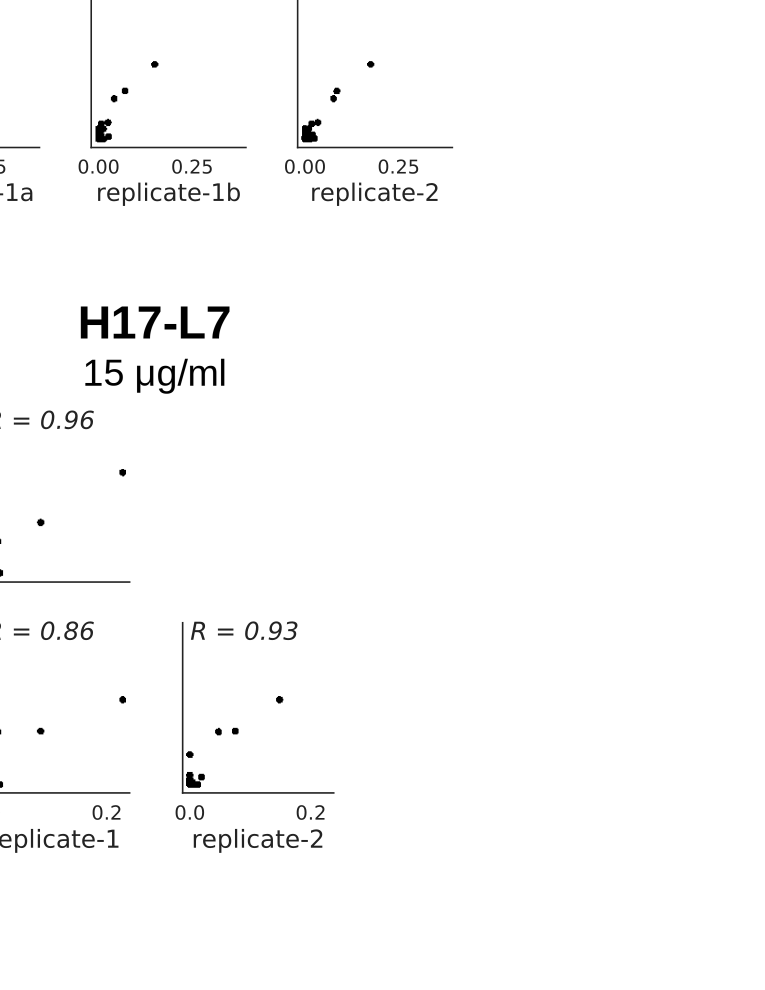
\includegraphics[width=0.5\textwidth]{figs/corrs/site_correlations_H17LAbs.pdf}}
\caption{\label{suppfig:corr}
Correlation of measurements across replicates. 
Each point represents one site in HA, and gives the fraction of mutant virions surviving selection taken across all amino-acid mutations at that site.
\comment{Elaborate after writing formula in METHODS.}
}
\end{suppfigure}

\begin{suppfigure}
\centerline{\includegraphics[width=\textwidth]{figs/maxfracsurvive.pdf}}
\caption{\label{suppfig:maxfracsurvive}
CAPTION}
\end{suppfigure}

\begin{suppfigure}
\centerline{\includegraphics[trim=0.1cm 0.02cm 0.1cm 0.03cm,clip=true,width=\textwidth]{figs/logoplots/H17L19_fracsurvive.pdf}}
\caption{\label{suppfig:H17L19logo}
CAPTION}
\end{suppfigure}

\begin{suppfigure}
\centerline{\includegraphics[trim=0.1cm 0.02cm 0.1cm 0.03cm,clip=true,width=\textwidth]{figs/logoplots/H17L10_fracsurvive.pdf}}
\caption{\label{suppfig:H17L10logo}
CAPTION}
\end{suppfigure}

\begin{suppfigure}
\centerline{\includegraphics[trim=0.1cm 0.02cm 0.1cm 0.03cm,clip=true,width=\textwidth]{figs/logoplots/H17L7_fracsurvive.pdf}}
\caption{\label{suppfig:H17L7logo}
CAPTION}
\end{suppfigure}

\end{document}
